\section{Problem A}
	\subsection{Statement}
        Given a graph and a spanning tree of the graph, determine whether the spanning tree is a valid BFS
        tree of the graph (rooted at $1$).

	\subsection{Solution}
        First, an obvious necessary condition is that the distances of each vertex should be the same in the graph
        and the tree.

        Rather lazily, we ask ``Is this condition also sufficient?''.

        Let's see for example the graph $G$ with the vertex set
        $V = \left\{1, 2, 3, 4, 5\right\}$ and the edge set 
        $E = \left\{12, 13, 24, 25, 35\right\}$.

        And consider the spanning tree $T$ with the edge set
        $E' = \left\{12, 13, 24, 35\right\}$, so the parents
        of $4$ and $5$ are $2$ and $3$ respectively.

        \begin{figure}[h]
        \centering
        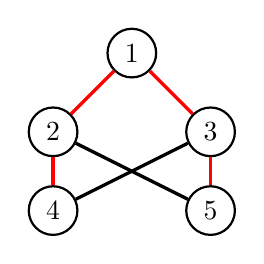
\begin{tikzpicture}
        \begin{scope}[every node/.style={circle, thick, draw}]
            \node (v1) at (2.5, 4) {1};
            \node (v2) at (1.5, 3) {2};
            \node (v3) at (3.5, 3) {3};
            \node (v4) at (1.5, 2) {4};
            \node (v5) at (3.5, 2) {5};
        \end{scope}

        \begin{scope}[
            every edge/.style={draw=red,very thick}]
            \path [-] (v1) edge (v2);
            \path [-] (v1) edge (v3);
            \path [-] (v2) edge (v4);
            \path [-] (v3) edge (v5);
            
        \end{scope}

        \begin{scope}[
            every edge/.style={draw=black,very thick}]
            \path [-] (v2) edge (v5);
            \path [-] (v3) edge (v4);

        \end{scope}
        \end{tikzpicture}
        \caption{The graph $G$, with the edges of $T$ in red} \label{Fig1}
        \end{figure}

        By examining the figure, you can see that $T$ is not a BFS-tree, so the obvious necessary
        condition is not sufficient $\ddot\smallfrown$